\PassOptionsToPackage{warn}{textcomp}

\documentclass[12pt,a4paper]{article}
\usepackage{amsmath, amssymb}
%\usepackage[warn]{mathtext}
\usepackage[T2A]{fontenc}
\usepackage[utf8]{inputenc} 
\usepackage[russian]{babel} 

\usepackage{textcomp}
%\DeclareSymbolFont{T2Aletters}{T2A}{cmr}{m}{rm}
\usepackage{epstopdf}
\usepackage[lastpage,user]{zref}
\usepackage{geometry, graphics, graphicx}

\geometry
{
	a4paper,
	total={210mm,297mm},
	left=20mm,
	right=20mm,
	top=25mm,
	bottom=20mm,
}

\usepackage{hyperref}

\hypersetup{
	    bookmarks=true,         % show bookmarks bar?
	%    unicode=false,          % non-Latin characters in Acrobat’s bookmarks
	%    pdftoolbar=true,        % show Acrobat’s toolbar?
	%    pdfmenubar=true,        % show Acrobat’s menu?
	%    pdffitwindow=false,     % window fit to page when opened
	%    pdfstartview={FitH},    % fits the width of the page to the window
	%    pdftitle={My title},    % title
	%    pdfauthor={Author},     % author
	%    pdfsubject={Subject},   % subject of the document
	%    pdfcreator={Creator},   % creator of the document
	%    pdfproducer={Producer}, % producer of the document
	%    pdfkeywords={keyword1, key2, key3}, % list of keywords
	%    pdfnewwindow=true,      % links in new PDF window
		colorlinks=true,       % false: boxed links; true: colored links
		linkcolor=blue!80!black,          % color of internal links (change box color with linkbordercolor)
		citecolor=green!30!black,        % color of links to bibliography
		filecolor=magenta!801black,      % color of file links
		urlcolor=blue!50!black           % color of external links
}

\usepackage{color}
\usepackage[usenames,table]{xcolor}

\colorlet{linkequation}{red!80!black}

\newcommand*{\SavedEqref}{}
\let\SavedEqref\eqref
\renewcommand*{\eqref}[1]{%
	\begingroup
	\hypersetup{
		linkcolor=linkequation,
		linkbordercolor=linkequation,
	}%
	\SavedEqref{#1}%
	\endgroup
}



% ----------------------------------------
% ------------Колонтитулы-----------------
\usepackage{fancyhdr}
\pagestyle{fancy}

\fancyhead{}
\rhead{\textbf{Выпонила:\\} \emph{Кузина Мария}}
\chead{\textsf{СПбПУ}\\им. Петра Великого}
\lhead{\textbf{Практическое задание №2\\} \emph{вариант 12}}
\lfoot{\scriptsize
	\textbf{UPD.:}~\emph{\today}\quad	
}
\cfoot{}
\rfoot{\thepage /\zpageref{LastPage}}

%% Листинги
%\definecolor{MatlabCellColour}{RGB}{252,251,220}
%\definecolor{mygreen}{RGB}{28,172,0} % color values Red, Green, Blue
%\definecolor{mylilas}{RGB}{170,55,241}
%\usepackage{listings}

\usepackage[framed,numbered,autolinebreaks,useliterate]{mcode}


%% Операторы
\usepackage{amsmath, amsopn}
\DeclareMathOperator{\sigm}{sigm}

\usepackage{hyperref}
\usepackage{diffcoeff}
\usepackage[final]{showlabels}

\usepackage{upgreek}
\newcommand{\del}{\Updelta}

\usepackage[labelsep=period]{caption}
\usepackage{float}

\newcommand{\ffnn}{\texttt{FFNN}}
\newcommand{\ff}{\texttt{FF}}
\newcommand{\hn}{\texttt{HN}}
\newcommand{\ns}{\texttt{Ns}}

%\renewcommand{\thesection}{\Asbuk{section}}
\renewcommand{\appendixname}{Приложение}

\usepackage{diffcoeff}
%\usepackage{enumitem}
%\renewcommand{\labelitemii}{\textopenbullet}

\renewcommand{\v}{\mathbf}

\usepackage{pgfplots}
\usetikzlibrary{calc}
\usetikzlibrary{graphs,graphs.standard}
\tikzgraphsset{declare={polygon_n}{[clique]\foreach\x in\tikzgraphV{\x/}}}
\usetikzlibrary{shapes.geometric}


\begin{document}
\section*{\Large\center Реализация нейронной сети Хопфилда
для анализа и классификации геометрических фигур}    
\section*{Условие}
\noindent
Написать программу моделирования нейронных сетей (НС) 
заданного типа и показать их работоспособность на практических примерах использования НС для указанной задачи.
Параметры НС представлены в таблице \ref{tbl:01}.

\begin{table}[h]
	\center
	\caption{Параметры модели \label{tbl:01}}
\begin{tabular}{lc|l}
\textbf{Вход} & & Изображения на некотором фоне одной из 5 геометрических фигур \\
\textbf{Выход} & & Какая фигура \\
\textbf{Тип НС} & & сеть Хопфилда \\
\textsf{\ns} &  & Число элементов в скрытом слое
\end{tabular}
\end{table}

\section{Постановка задачи, связанной с практическим \newline применением НС}
Компьютерное зрение на основе методов распознавания геометрической 
формы получило широкое распространие на производстве в таких областях 
как промышленный осмотр, идентификация, и автоматический контроль
качества продукции. 
В задаче автоматической сборки, значительный объем информации о детали
необходимо распознавать и классифицировать, а ее ориентация должна быть 
автоматически определена, прежде чем робот (манипулятор) сможет ухватиться 
за изделие или его часть. 
Также применяются методы распознавания формы
для оптического распознавания символов, рукописного текста,
а также медицинских изображений, и.т.д. \cite{hou1999}.\\[6pt]
\noindent
\emph{Базовой задачей}, предваряющей перечисленные выше является
задача распознавания и классификации плоских геометрических фигур
таких как треугольник, квадрат, пентагон, шестиугольник и круг 
(многоугольник с количеством сторон $\sim100$).

\section{Описание теоретической базы рассматриваемой \newline модели НС}
Сеть Хопфилда представляет собой однослойную полносвязную нейронную сеть с симметричной матрицей связей \cite{hopfield1982}. 
Каждый нейрон может принимать как на входе, так и на выходе лишь одно из двух состояний $\{1,\,-1\}$ . 
Рассмотрим схему сети Хопфилда с тремя нейронами, представленную на
рис.\,\ref{fig:01}. Выход каждого из нейронов замыкается (обратная связь) на вход всех остальных нейронов сети.

%Во время получения 
%входных данных каждый узел является входом, в процессе обучения 
%он становится скрытым, а затем становится выходом. 
%Сеть обучается так: значения нейронов устанавливаются в соответствии 
%с желаемым шаблоном, после чего вычисляются веса, которые в дальнейшем 
%не меняются. После того, как сеть обучилась на одном или нескольких шаблонах, 
%она всегда будет сводиться к одному из них (но не всегда к желаемому). 
%Она стабилизируется в зависимости от общей «энергии» и «температуры» сети. 
%У каждого нейрона есть свой порог активации, зависящий от температуры, 
%при прохождении которого нейрон принимает одно из двух значений 
%(обычно $-1$ или $1$, иногда 0 или 1).  Такая сеть часто называется сетью 
%с ассоциативной памятью; как человек, видя половину таблицы, может 
%представить вторую половину таблицы, так и эта сеть, получая таблицу, 
%наполовину зашумленную, восстанавливает её до полной.

\begin{figure}[h!]
	\centering
	\includegraphics[height=0.4\textheight]{_ref_/hopfield/1}
	\caption{Схема сети Хопфилда\label{fig:01}}
\end{figure}



Пусть $W$ есть матрица связей сети Хопфилда с $\ns$ нейронами, тогда
\begin{equation*}
W = 
\begin{pmatrix}
0 & \ldots & w_{1\ns} \\
\vdots & \ddots & \vdots \\
w_{\ns 1} & \ldots & 0
\end{pmatrix},
\quad
w_{1\ns} = w_{\ns 1}.
\end{equation*}

Построенная таким образом нейронная сеть обладает свойством конвергенции, т.е. конечным (мощностью $M$) множеством положений равновесия, к которым сеть будет сходиться в своей динамике. 
Под динамикой в данном случае будем иметь в виду итеративный 
(например, $I: 1\rightarrow500$) процесс преобразования вектора входных значений $X_{\xi}$ размерности $\ns$ ($\ns$ равно общему числу нейронов) к некоторому выходному вектору $Y_{\xi}$ той же размерности. 
Причём, если $X_i$ -- положение равновесия, то
\begin{equation}\label{eq:01}
X_i = WX_i.
\end{equation}
В случае, когда $X_{\xi} = X_i - \varepsilon$ имеем
$$
WX_{\xi}\rightarrow Y_{\xi}=X_i.
$$	
Для сетей с обратными связями симметричность и нули на главной 
диагонали матрицы связей представляют собой необходимое условие \cite{hopfield1982} существования устойчивых положений равновесия 
(некое положение равновесия называют устойчивым, если рассматриваемая система, оказавшись в этом положении, стремится в нём и остаться). 
В случае сетей Хопфилда достаточным условием устойчивости сети 
будет т.н. асинхронный (в отличии от синхронного) режим работы. 
При соблюдении необходимого, но не достаточного условий устойчивости, возможен переход к динамическому аттрактору: ситуации, при которой 
сеть бесконечно (т.е. с каждой новой итерацией) переключается между
двумя своими разными состояниями.

Отличие синхронного и асинхронного режимов работы заключается в способе обсчета новых состояний нейронов сети. При синхронном режиме нейроны просматриваются последовательно, однако их текущие состояния запоминаются отдельно и не меняются до тех пор, пока не будут пройдены все нейроны сети. В асинхронном режиме текущее состояние заменяется новым ещё до прохода по всем нейронам.

Процесс обучения сети Хопфилда заключается в построении такой матрицы связей $W$, чтобы все запоминаемые вектора--образы $X_i$ оказались устойчивыми положениями равновесия \eqref{eq:01}. Если все запоминаемые векторы имеют бинарный вид, то матрица $W$ может быть найдена вычислением внешнего произведения каждого запоминаемого вектора с самим собой и суммированием матриц, полученных таким образом в виде
$$
W = \dfrac{1}{\ns}\sum\limits_i X_iX_i^T.
$$

Алгоритм обучения сети Хопфилда существенно отличается от таких классических алгоритмов обучения перцептронов, как метод коррекции ошибки или метод обратного распространения ошибки. Отличие заключается в том, что вместо последовательного приближения к нужному состоянию с вычислением ошибок, все коэффициенты матрицы рассчитываются по одной формуле, за один цикл, после чего сеть сразу готова к работе.



\section{Описание разработанных ПМ и решение задачи}
Были рассмотрены четыре геометрические фигуры, являющиеся правильными выпуклыми $n-$угольниками: треугольник, квадрат, пятиугольник и шестиугольник. В качестве пятой фигуры был рассмотрен правильный 
$100-$угольник (аналог круга). См. рис.\,\ref{fig:02}.\\



\begin{figure}[tbh!]
	\center
	\newdimen\R
	\R=.65cm
	\begin{tikzpicture}
	% Indicate the boundary of the regular polygons
	\draw[fill=red!25] (0:\R) \foreach \x in {120,240} {
		-- (\x:\R)
	} -- cycle (90:\R);
	\draw[fill=green!25,xshift=2.5\R] (0:\R) \foreach \x in {90,180,...,359} {
		-- (\x:\R)
	} -- cycle (90:\R);
	\draw[fill=blue!25,xshift=5.0\R] (0:\R) \foreach \x in {72,144,...,359} {
		-- (\x:\R)
	} -- cycle (90:\R);
	\draw[fill=magenta!25,xshift=7.5\R] (0:\R) \foreach \x in {60,120,...,359} {
		-- (\x:\R)
	}-- cycle (90:\R);
	\draw[fill=black!25,xshift=10.0\R] (0:\R) \foreach \x in {3.6,7.2,...,359} {
		-- (\x:\R)
	} -- cycle (90:\R);
	\end{tikzpicture}
	\caption{Геометрические фигуры, на которых обучалась НС}
	\label{fig:02}
\end{figure}

\noindent
Сформированы обучающие и соответствующие им тестовые выборки.\\[6pt]

\begin{figure}[tbh!]
	\centering
	\includegraphics[scale=0.125]{_ref_/3-gone-smpl}	
	\includegraphics[scale=0.125]{_ref_/4-gone-smpl}
	\includegraphics[scale=0.430]{_ref_/5-gone-smpl}	
	\includegraphics[scale=0.125]{_ref_/6-gone-smpl}	
	\includegraphics[scale=0.125]{_ref_/100-gone-smpl}						
	\caption{Примеры сгенерированных фигур}
	\label{fig:03}
\end{figure}

\noindent
Выборка \textnumero\,1 содержит изображения пяти указанных геометрических фигур, с фиксированными положением, размером и цветом. 
От изображения к изображению меняется только цвет фона.\\[6pt]
\noindent
Выборка \textnumero\,2 содержит изображения с фигурами разной площади 
и цвета заливки. Введён случайный угол поворота фигуры. 
Цвет фона изображения также меняется.\\[6pt]

\begin{figure}[H]
	\centering
	\includegraphics[scale=0.95]{_ref_/hopfield/2}					
	\caption{Зашумленный пятиугольник}
	\label{fig:04}
\end{figure}

\noindent
Выборка \textnumero\,3 представляет собой выборку \textnumero\,1 
с той разницей, что на некоторые изображения наложен гауссовский шум с максимальным уровнем 0.5. Пример изображения представлен 
на рис.\,\ref{fig:04}.

\subsubsection*{Файлы \texttt{Matlab}:}
\verb|gen_set_of_ngons.m|\\
\verb|gen_ngon_image.m|\\
\verb|run_gen_ngon.m|\\[6pt]

\noindent
Поскольку сеть Хопфилда может работать лишь с массивами бинарных 
данных, имеющиеся изображения необходимо приводить к соответствующему виду. Для этого переведём изображение (изначально 3 канала)
$$
R\in[0,\,255],~G\in[0,\,255],~B\in[0,\,255]
$$
в оттенки серого 
$$
R = G = B = x,
$$ 
преобразуем его в одномерный 1D -- массив. 
Далее приведём полученные значения к диапазону от $-1$ до $1$. 
Все имеющиеся значения округлим по следующему правилу:\\ 
значения от $-1$ до 0 приравняем к $-1$, \\
значения от 0 до 1 приравняем к 1.

На рис.\,\ref{fig:05} показан результат перечисленных действий в применении к изображению ромба (квадрата) (без преобразования к одномерному массиву).

\begin{figure}[H]
	\centering
	\includegraphics[width=0.5\textwidth]{_ref_/hopfield/3}		
	\caption{Ромб (квадрат)}
	\label{fig:05}
\end{figure}

Указанным выше способом сформируем пять примеров--эталонов для 
всех имеющихся фигур и обучим на таких примерах сеть Хопфилда. 
Количество нейронов в сети будет варьироваться в зависимости от 
размера изображения (высота $\times$ ширина попиксельно). 
В данной работе использовались изображения 
$28\times28$ и $50\times50$. Вход--выход: 784---784 и 2500---2500 соответственно. 

Сконфигурированная и обученная таким образом сеть показывает близкие к 100\% результаты на выборках \textnumero\,1 и \textnumero\,3. 
Каждое изображение из тестового набора изображений (500 примеров) было верно проассоциировано с эталоном. Действительно, сети Хопфилда удачно применяют наряду со множеством существующих шумоподавляющих фильтров, рис.\ref{fig:06}.

\begin{figure}[H]
	\centering
	\includegraphics[height=3cm]{_ref_/hopfield/04}	\quad	
	\includegraphics[height=3cm]{_ref_/hopfield/03}		
	\caption{Пример эталонного изображения и изображения с шумом}
	\label{fig:06}
\end{figure}

\noindent
На ''сложной'' выборке \textnumero\,2 распознавание едва превысило 
$5\sim12\%$.

В рамках эксперимента и с целью улучшения качества распознавания 
фигур, была предпринята попытка обучить сеть Хопфилда не на 
самих изображениях эталонных фигур, а на их спектрах Фурье. 
Приведение исходных изображений к их 2D--спектрам решает 
проблему произвольного положения фигуры относительно центра 
изображения в выборке \textnumero\,2: достаточно сместить 
полученный Фурье--спектр по нулевой частоте. 
Форма 2D--спектра определённой фигуры меняется в зависимости от поворота 
этой фигуры: некоторые линии утолщаются и немного сдвигаются, 
другие -- наоборот. 
Однако формы спектров одних и тех же фигур продолжают оставаться визуально схожими, тогда как для различных фигур различия формы сохраняются.

\begin{figure}[H]
	\centering
	\begin{minipage}[h]{0.29\linewidth}
		\center{\includegraphics[width=0.85\linewidth]{_ref_/hopfield/4-1} \\ а) треугольник}
	\end{minipage}
	\hfill
	\begin{minipage}[h]{0.29\linewidth}
		\center{\includegraphics[width=0.85\linewidth]{_ref_/hopfield/4-2} \\ б) квадрат}
	\end{minipage}
	\hfill
	\begin{minipage}[h]{0.29\linewidth}
		\center{\includegraphics[width=0.85\linewidth]{_ref_/hopfield/4-3} \\ в) круг}
	\end{minipage}
		\vfill
	\begin{minipage}[h]{0.49\linewidth}
		\center{\includegraphics[width=0.5\linewidth]{_ref_/hopfield/4-4} \\ г) пятиугольник}
	\end{minipage}
		\hfill
	\begin{minipage}[h]{0.49\linewidth}
		\center{\includegraphics[width=0.5\linewidth]{_ref_/hopfield/4-5} \\ д) шестиугольник}
	\end{minipage}
	\caption{Спектры фигур из множества эталонных примеров}
	\label{fig:07}
\end{figure}

\noindent
После обучения сети и её проверки на тестовых наборах изображений процент распознавания вырос всего до 30\%.
Сеть Хопфилда в динамике представлена на рис.\,\ref{fig:08}.

\begin{figure}[H]
	\centering
	\begin{minipage}[h]{0.49\linewidth}
		\center{\includegraphics[width=0.7\linewidth]{_ref_/hopfield/dynamic/01000} \\ а) тестовый пример}
	\end{minipage}
	\hfill
	\begin{minipage}[h]{0.49\linewidth}
		\center{\includegraphics[width=0.7\linewidth]{_ref_/hopfield/dynamic/1} \\ б) итерация 1}
	\end{minipage}
	\hfill
	\begin{minipage}[h]{0.49\linewidth}
		\center{\includegraphics[width=0.7\linewidth]{_ref_/hopfield/dynamic/2} \\ в) итерация 2}
	\end{minipage}
	\hfill
	\begin{minipage}[h]{0.49\linewidth}
		\center{\includegraphics[width=0.7\linewidth]{_ref_/hopfield/dynamic/3} \\ г) итерация 3}
	\end{minipage}
	\hfill
	\begin{minipage}[h]{0.49\linewidth}
		\center{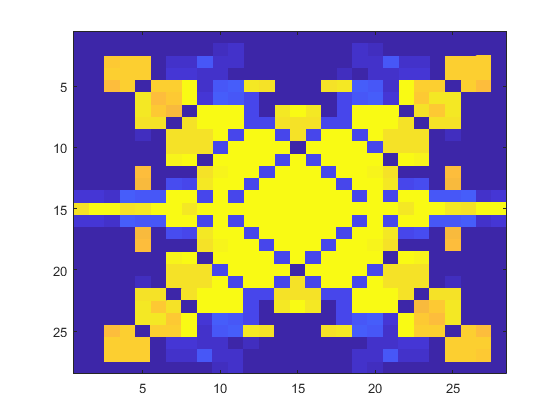
\includegraphics[width=0.7\linewidth]{_ref_/hopfield/dynamic/4} \\ д) итерация 4}
	\end{minipage}
	\hfill
	\begin{minipage}[h]{0.49\linewidth}
		\center{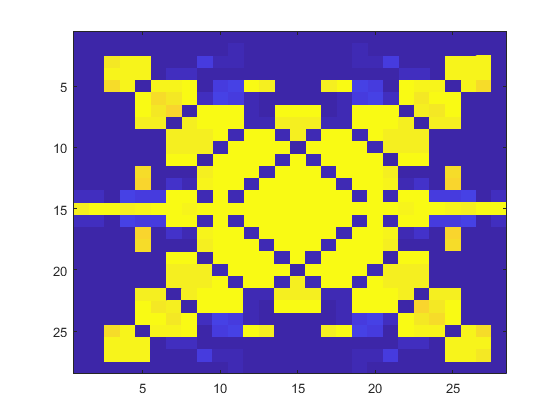
\includegraphics[width=0.7\linewidth]{_ref_/hopfield/dynamic/5} \\ е) итерация 5}
	\end{minipage}
	\hfill
	\begin{minipage}[h]{0.49\linewidth}
		\center{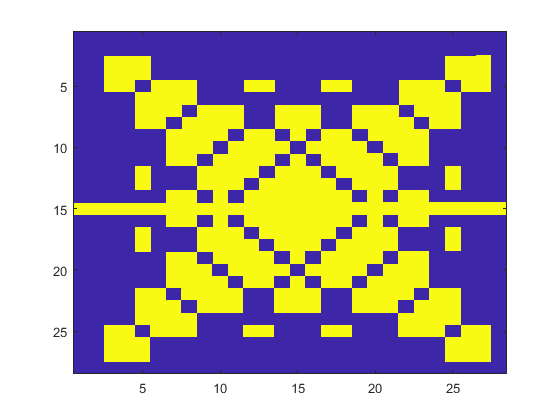
\includegraphics[width=0.7\linewidth]{_ref_/hopfield/dynamic/6} \\ ё) итерация 6}		
	\end{minipage}
	\hfill
	\begin{minipage}[h]{0.49\linewidth}
		\center{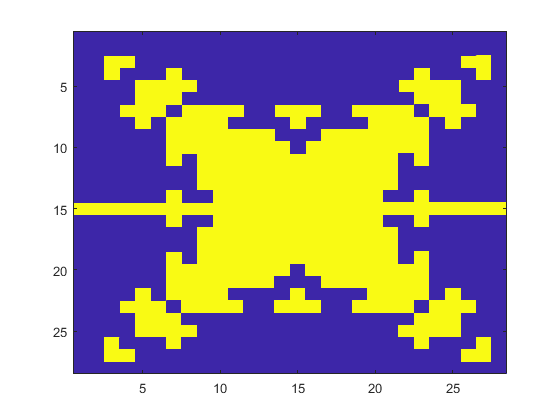
\includegraphics[width=0.7\linewidth]{_ref_/hopfield/dynamic/0} \\ ё) итерация 7}		
	\end{minipage}
	\caption{Итерационный процесс для сети Хопфилда}
	\label{fig:08}
\end{figure}

\subsubsection*{Файлы \texttt{Matlab}:}
\verb|load_dataset.m |\\
\verb|load_testdataset.m |\\
\verb|create_net.m|\\
\verb|test_net.m|\\[6pt]





\newpage
\section{Альтернативные способы решения}
%Альтернативные способы решения рассматриваемой задачи и сравнение с нейросетевым подходом (отразить достоинства, недостатки, возможные ограничения на постановку задачи и требования по априорной информации для формирования обучающих примеров).
Альтернативными являются два подхода классификации фигур, которые во многом противоположны друг другу.\\
\noindent
\textbf{Первым подходом} является подход на основе спектрального анализа \cite{direkoglu2011}. 
Представление формы объекта на основе \emph{Фурье дескрипторов} легко организовать в плане вычислений,
а результаты будут устойчивы к внешнему шуму. Фурье дескрипторы получаются при помощи преобразования
Фурье, применённого к \emph{сигнатуре формы объекта}, границе объекта как одномерной функции.


\begin{figure}[tbh!]
	\center
	\includegraphics[scale=0.5]{_ref_/direkoglu2011_fig}
	\caption{Пример обработки изображения лошади \cite{direkoglu2011}}
%	\label{fig:08}
\end{figure}
Существуют и другие сигнатуры формы, например, расстояние от центра объекта (в пикселях) до остальных пикселей,
кривизна границы и кумулятивный угол. Геометрические характеристики (инварианты) объекта
определяются на этапе определения сигнатуры формы объекта, который может происходить как до
Фурье преобразования, так и после. При этом, нижние частоты дескрипторов содержат
информацию о форме объекта, а верхние частоты о деталях.

\noindent
\textbf{Вторым подходом} является геометрический подход, который предполагает выделение контура \cite{wang2014}. 
Он основывается на разработке дескрипторов формы малого разрешения, которые могут быть
устойчивы к поворотам, масштабированию и деформации объекта.

\begin{figure}[H]
	\center
	\includegraphics[scale=0.44]{_ref_/xinggang2014_fig}
	\caption{Пример обработки изображения бабочки \cite{wang2014}}
%	\label{fig:08}
\end{figure}

В таком подходе граница объекта разбивается на составные части (сегменты), каждая
из которых далее описывается при помощи того или иного дескриптора. После чего
для решения задачи классификации применяются методы машинного обучения, например,
метод опорных векторов \cite{svm}.


\section{Области применения НС заданного типа}
Ассоциативность памяти нейронной сети Хопфилда является не единственным ее прктическим свойством. 
Другим важным свойством этой архитектуры является уменьшение ее функции Ляпунова в процессе нейродинамики. Отсюда, сеть Хопфилда можно рассматривать как алгоритм оптимизации целевой функции в форме энергии сети.

Класс целевых функций, которые могут быть минимизированы нейронной сетью достаточно широк: в него попадают все билинейные и квадратичные формы с симметричными матрицами.

Сюда относятся такие традиционные задачи, как дифференциальные уравнения в вариационной постановке; задачи линейной алгебры и системы нелинейных алгебраических уравнений, где решение ищется в форме минимизации невязки, и другие.

Помимо того, что сеть Хопфилда может быть использована как автоассоциативная память, и для решения некоторых задач оптимизации,
она также может быть использована как фильтр. 

\newpage
\appendix 
\addcontentsline{toc}{section}{Список литературы}


\begin{thebibliography}{99}
\bibitem{hopfield1982} J.J. Hopfield, Neural Networks and Physical Systems with Emergent Collective Computational Abilities. Proc. NatL Acad. Sci. USA, Vol. 79, 1982, pp. 2554--2558. \textbf{DOI:~:10.1073/pnas.79.8.2554}

\bibitem{cohen1983} Cohen M.A., Grossberg S.G., Absolute stability of global pattern formation and parallel memory storage by compatitive neural networks. IEEE Transactions on Systems, Man and Cybernetics, Vol. 13, 1983, pp. 815--26. \textbf{DOI:~:10.1109/TSMC.1983.6313075}
%
%\bibitem{NNzoo} Шпаргалка по разновидностям нейронных сетей. Часть первая. Элементарные конфигурации. \textbf{URL:~\url{https://tproger.ru/translations/neural-network-zoo-1/}}
%
%\bibitem{FFNNsample} A simple example of feedforward neural network and image recognition.
%\textbf{URL:~\url{https://dummas.wordpress.com/2012/01/14/a-simple-example-of-feedforward-neural-network-with-image-recognition/}}

\bibitem{hou1999} Tung-Hsu Hou and Ming-Der Pern, A Computer Vision-Based Shape-Classification System Using
Image Projection and a Neural Network.
Int. J. Adv. Manuf. Technol., 15, 1999, pp. 843--850.
\textbf{DOI:~10.1007/s001700050141}

\bibitem{direkoglu2011} Cem Direko\u{g}lu, Mark S. Nixon, Shape classification via image-based multiscale description.
Pattern Recognition, 44, 2011, pp. 2134--2146. \textbf{DOI:~10.1016/j.patcog.2011.02.016}

\bibitem{wang2014} Xinggang Wang, Bin Feng, et.al., Bag of contour fragments for robust shape classification.
Pattern Recognition, 47, 2014, pp. 2116--2125. \textbf{DOI:~10.1016/j.patcog.2013.12.008}

\bibitem{svm} К.В. Воронцов. Лекции по методу опорных векторов. \textbf{URL:~\url{http://www.ccas.ru/voron/download/SVM.pdf}}

\end{thebibliography}


\newpage
\appendix 
\addcontentsline{toc}{section}{Тексты программ}

\section*{Тексты программ}
\verb|test_net.m|
\begin{lstlisting}
steps = 500;
[Y_img, Pf1, Af1, E1, perf1] = sim(net_img, {steps}, [], TestImages(:, 5));
% [Y_fft, Pf2, Af2, E2, perf2] = sim(net_fft, {steps}, [], TestFFTs(:, 2));

imagesc(reshape(Y_img{1, steps}, [hvP_size, hvP_size]));
% imagesc(reshape(Y_fft{1, steps}, [hvP_size, hvP_size]));
\end{lstlisting}

\noindent
\verb|create_net.m|
\begin{lstlisting}
% newhop - Hopfield network create
net_img = newhop(Images);
net_fft = newhop(FFTs);
\end{lstlisting}

\noindent
\verb|load_dataset.m|
\begin{lstlisting}
triangleFolder = '_img_/3-gone/';       % label: 1
rectangleFolder = '_img_/4-gone/';      % label: 2
circleFolder = '_img_/100-gone/';       % label: 3
pentagonFolder = '_img_/5-gone/';       % label: 4
hexagonFolder = '_img_/6-gone/';        % label: 5

% getting filelists 
dirData = dir(triangleFolder);
dirIndex = [dirData.isdir];
fileListTriangles = {dirData(~dirIndex).name}';
dirData = dir(rectangleFolder);
dirIndex = [dirData.isdir];
fileListRectangles = {dirData(~dirIndex).name}';
...

N = 1;
hvP_size = 28;
P_size = hvP_size * hvP_size;

trianglesI = zeros(P_size, N);
...
trianglesFFT = zeros(P_size, N);
...

for i = 1:N
  fpath = strcat(triangleFolder, fileListTriangles{i});
  disp(fpath);
  I = imread(fpath);
  I = imresize(I, [hvP_size hvP_size]);
  II = reshape(I(:,:,1), [P_size, 1]);    
  trianglesI(:, i) = II;
  I = fft2(I);
  I = reshape(abs(fftshift(I(:,:,1))), [P_size,1]);
  trianglesFFT(:, i) = I;

  fpath = strcat(rectangleFolder, fileListRectangles{i});
  disp(fpath);
  I = imread(fpath);
  I = imresize(I, [hvP_size hvP_size]);
  II = reshape(I(:,:,1), [P_size, 1]);
  rectanglesI(:, i) = II;
  I = fft2(I);
  I = reshape(abs(fftshift(I(:,:,1))), [P_size,1]);
  rectanglesFFT(:, i) = I;

...
end

N5 = 5 * N;
DataSet_Images_Total = zeros(1, P_size, N5);
DataSet_FFTs_Total = zeros(1, P_size, N5);

%% Total
k = 1;
for i = 1:N
  DataSet_Images_Total(1,:,k) = trianglesI(:, i);
  DataSet_FFTs_Total(1,:,k) = trianglesFFT(:, i);
  k = k + 1;

  DataSet_Images_Total(1,:,k) = rectanglesI(:, i);
  DataSet_FFTs_Total(1,:,k) = rectanglesFFT(:, i);
  k = k + 1;

...
end

Images = squeeze(DataSet_Images_Total(1, :, :));
FFTs = squeeze(DataSet_FFTs_Total(1, :, :));
for i = 1:P_size
  for j = 1:N5
    Images(i, j) = round(Images(i, j)/256);
    if (Images(i, j) == 0)
      Images(i, j) = -1;
    end
    if (Images(i, j) > 1)
      Images(i, j) = 1;
    end
    FFTs(i, j) = round(FFTs(i, j)/256);
    if (FFTs(i, j) == 0)
      FFTs(i, j) = -1;
    end
    if (FFTs(i, j) > 1)
      FFTs(i, j) = 1;
    end
  end
end

I = reshape(Images(:, 5), [hvP_size, hvP_size]);
imagesc(I);
%% I = reshape(FFTs(:, 5), [hvP_size, hvP_size]);
%% imagesc(I);
%\end{lstlisting}

\noindent
\verb|load_testdataset.m|
\begin{lstlisting}
triangleFolder = '_img_/TEST/3-gone/';       % label: 1
rectangleFolder = '_img_/TEST/4-gone/';      % label: 2
circleFolder = '_img_/TEST/100-gone/';       % label: 3
pentagonFolder = '_img_/TEST/5-gone/';       % label: 4
hexagonFolder = '_img_/TEST/6-gone/';        % label: 5

% getting filelists 
dirData = dir(triangleFolder);
dirIndex = [dirData.isdir];
fileListTriangles = {dirData(~dirIndex).name}';
...

N = 20;

trianglesI = zeros(P_size, N);
...
trianglesFFT = zeros(P_size, N);
...

for i = 1:N
fpath = strcat(triangleFolder, fileListTriangles{i});
disp(fpath);
I = imread(fpath);
I = imresize(I, [hvP_size hvP_size]);
II = reshape(I(:,:,1), [P_size, 1]);    
trianglesI(:, i) = II;
I = fft2(I);
I = reshape(abs(fftshift(I(:,:,1))), [P_size,1]);
trianglesFFT(:, i) = I;

fpath = strcat(rectangleFolder, fileListRectangles{i});
disp(fpath);
I = imread(fpath);
I = imresize(I, [hvP_size hvP_size]);
II = reshape(I(:,:,1), [P_size, 1]);
rectanglesI(:, i) = II;
I = fft2(I);
I = reshape(abs(fftshift(I(:,:,1))), [P_size,1]);
rectanglesFFT(:, i) = I;

...
end

N5 = 5 * N;
TestDataSet_Images_Total = zeros(1, P_size, N5);
TestDataSet_FFTs_Total = zeros(1, P_size, N5);

% Total
k = 1;
for i = 1:N
TestDataSet_Images_Total(1,:,k) = trianglesI(:, i);
TestDataSet_FFTs_Total(1,:,k) = trianglesFFT(:, i);
k = k + 1;

TestDataSet_Images_Total(1,:,k) = rectanglesI(:, i);
TestDataSet_FFTs_Total(1,:,k) = rectanglesFFT(:, i);
k = k + 1;

...
end

TestImages = squeeze(TestDataSet_Images_Total(1, :, :));
TestFFTs = squeeze(TestDataSet_FFTs_Total(1, :, :));

for i = 1:P_size
for j = 1:N5
TestImages(i, j) = round(TestImages(i, j)/256);
if (TestImages(i, j) == 0)
TestImages(i, j) = -1;
end
if (TestImages(i, j) > 1)
TestImages(i, j) = 1;
end
TestFFTs(i, j) = round(TestFFTs(i, j)/256);
if (TestFFTs(i, j) == 0)
TestFFTs(i, j) = -1;
end
if (TestFFTs(i, j) > 1)
TestFFTs(i, j) = 1;
end
end
end

I = reshape(TestImages(:, 1), [hvP_size, hvP_size]);
imagesc(I);
% I = reshape(TestFFTs(:, 2), [hvP_size, hvP_size]);
% imagesc(I);
\end{lstlisting}

\newpage
%% Оглавление
\newpage
\tableofcontents

\end{document}